\documentclass{beamer}

\usepackage[main=english,finnish]{babel}
\usepackage{cmbright}
\usepackage{fontspec}
\usepackage{booktabs}
\usepackage{hyperref}
\usepackage{graphicx}
\usepackage{pifont}
\usepackage{layout}

\newcommand{\cmark}{\ding{51}}%
\newcommand{\xmark}{\ding{55}}%

\hypersetup{pdfencoding=auto}

\newsavebox{\mysavebox}
\newlength{\myrest}

%\usepackage{polyglossia}
\setsansfont[Ligatures = TeX,
             BoldFont  = CMU Bright SemiBold,
             ItalicFont = CMU Bright Oblique,
            ]{CMU Bright Roman}
\setmainfont[Ligatures = TeX,
             BoldFont  = CMU Bright SemiBold,
             ItalicFont = CMU Bright Oblique,
            ]{CMU Bright Roman}
\setmonofont[Ligatures = TeX,
             BoldFont  = CMU Typewriter Text Bold,
             ItalicFont = CMU Typewriter Text Oblique,
            ]{CMU Typewriter Text}
\usetheme{Madrid}

\mode<presentation>
\setbeamercovered{transparent}
\setbeamertemplate{enumerate items}[default]
\setbeamertemplate{itemize items}[default]

\title[Finnish language text mining]{Extraction, exploration and exploitation of diverse Finnish language texts}
\subtitle{TIES445 Data Mining project}
\author[Robertson \& Kanushin]{Frankie Robertson\inst{1} \and Max Kanushin\inst{2}}
\institute[JYU, LETI]{\inst{1} University of Jyväskylä \and%
                      \inst{2} Saint Petersburg State Electrotechnical University}

\date{18th of April, 2016}

\titlegraphic{
  \includegraphics[height=1.5cm]{jyu.pdf}
  \hspace{1cm}
  \includegraphics[height=1.5cm]{leti_logo.png}
}

\begin{document}

\section{Title}
\begin{frame}
  \titlepage{}
\end{frame}

\section{Contents}
\begin{frame}
\frametitle{Contents}
\begin{enumerate}
  \item Orientation and aims\pause{}
  \item Extraction (scraping + preprocessing)\pause{}
  \item Exploration (mainly visualisation through dimension reduction)\pause{}
  \item Exploitation (obtain metrics which could be useful for presentation directly to an end-user or for use within a larger application)
\end{enumerate}

\end{frame}

\section{Orientation \& aims}
\begin{frame}
\frametitle{Orientation}

\begin{itemize}
  \item The Finnish language is used in different ways in different contexts.\pause{}

  \item For Finnish in particular there is a marked difference between spoken and
        written Finnish.\pause{}

  \item There are more complex grammatical features of Finnish which are used
        only rarely (in particular many inflections are used only rarely).\pause{}

  \item Wouldn't it be nice to be able to distinguish between written and
        spoken and between less and more complex Finnish?
\end{itemize}

\end{frame}

\begin{frame}
\frametitle{Aims}

\begin{itemize}
  \item Create a data set which characterises the range of these two dimensions
        of Finnish. \textit{(Extraction)} \cmark{}\pause{}

  \item Create features based on this data set and visualise them.
        \textit{(Exploration)} \cmark{}\pause{}

  \item Create a model which can attempt to characterise unseen data.
        \textit{(Exploitation)} \xmark{} -- still at the ideas stage
\end{itemize}

\end{frame}

\section{Extraction}

\begin{frame}
\frametitle{Sources}

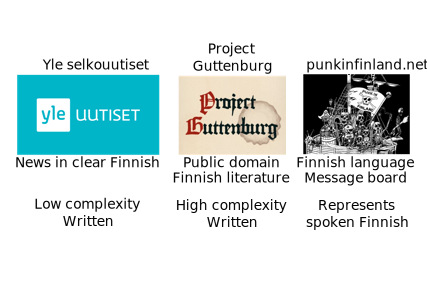
\includegraphics{sources.pdf}

\end{frame}

\begin{frame}
  \frametitle{Scraping \& data processing pipeline}
  \begin{columns}[onlytextwidth]
    \begin{column}{0.7\textwidth}
      \begin{itemize}
        \item We used Scrapy to write three custom spiders in Python. One key
          advantage of using Scrapy is that it makes it easy to write a reasonably
          well performing event based spider.\pause{}
        \item Another script converts the raw text into a series of matrices in a
          load'able .mat file in a similar format to the fisheriris data set.
          Different features of the data are stored in different matrices.
      \end{itemize}
    \end{column}
    \begin{column}{0.3\textwidth}
    
\includegraphics{pipeline.pdf}
    \end{column}
\end{columns}
\end{frame}

\begin{frame}
  \frametitle{Preprocessing \& feature extraction}
  \begin{itemize}
    \item One set of matrices stores distributions of word length and sentence
      length. Sentence and word tokenisation was performed with the Python
      module nltk.
    \item Lemmas were extracted with FinnPos which is a morphological analyser
      with guessing, disambiguation and part of speech tagging built on top of
      OMorFi which is a morphological database for Finnish. Theoretically it
      should be possible to segment word forms into morphs but for the sake of
      trying to get something working quickly, a lazy measure was used: the
      different between lemma length and word form length.
    \item Another set of matrices represents 
  \end{itemize}
\end{frame}

\begin{frame}
\frametitle{Aside/soap box: legality}

\begin{itemize}
  \item The legality of text mining on copyrighted material (which is pretty
    much everything recorded due to the Berne Convention) is unclear in the
    EU\pause{}
  \item In the US the recent Google Books case has cemented the the idea of a
    ``transformative factor'' of fair use (at least if you're Google)\pause{}
  \item Science Europe has published a detailed document about these issues:
    \href{http://www.scienceeurope.org/uploads/PublicDocumentsAndSpeeches/WGs_docs/SE_Briefing_Paper_textand_Data_web.pdf}%
    {Text and Data Mining and the Need for a Science-friendly EU Copyright Reform}\pause{}
  \item One of the recommendations is that research organisations should take a
    hands off approach and allow individual researchers to make their own
    choice as part of the process of pushing for new copyright exceptions
    rather than insisting on strict adherence to the obeying the letter of the
    law
\end{itemize}

\end{frame}

\end{document}
